\section{MOTOR INVARIANT CONTROL}
\begin{figure*}[t]
\centerline{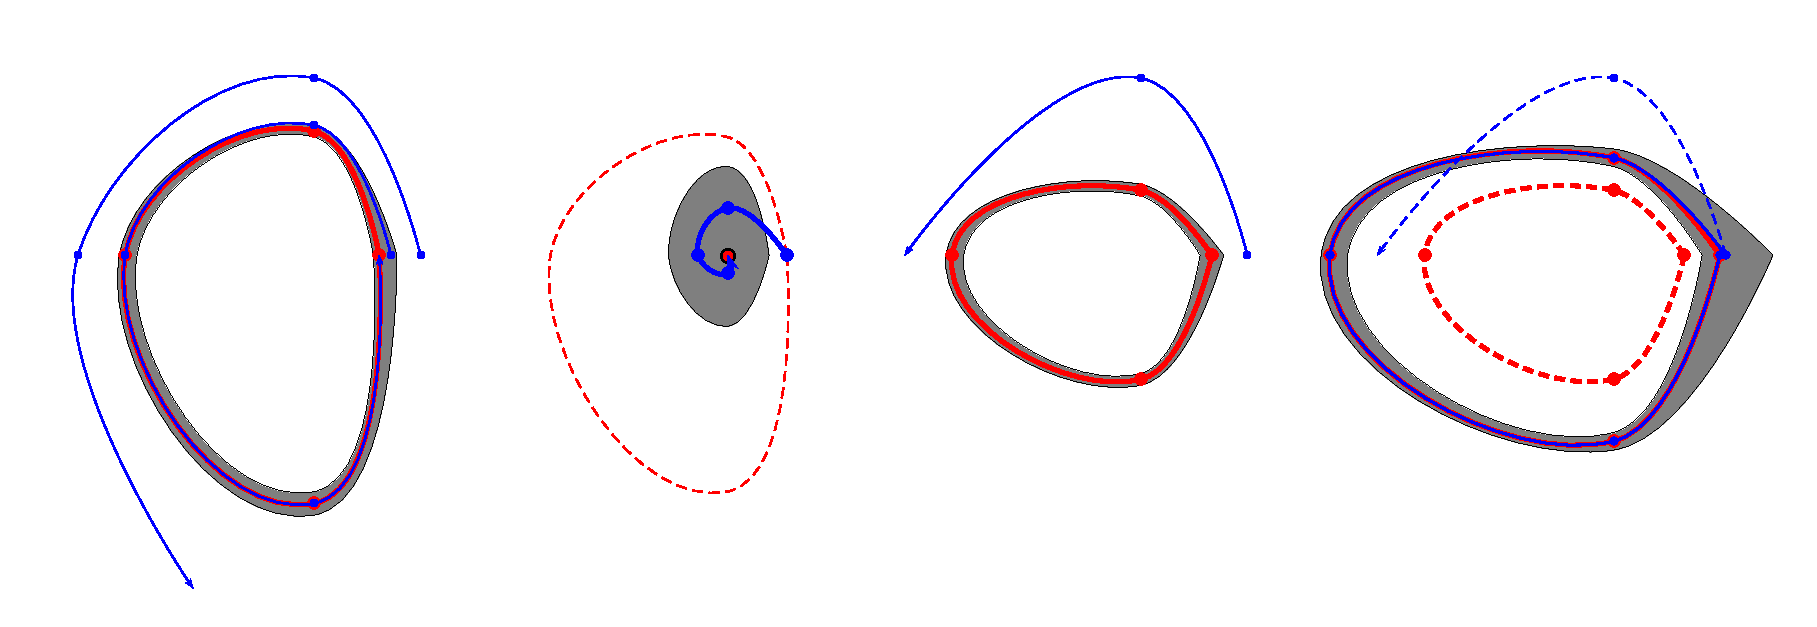
\includegraphics[width=11cm]{images/LimitCircle.eps}}
\caption{Comparison of the results predicted by our models against video of a human iris. (left) One frame of an
animation simulating the changes in pupil diameter and iridal pattern deformation. (center) One frame from a video of a
human iris. (right) Graph comparing the measured pupil diameters from each individual frame of a nine-second-long video
sequence (green line) against the behavior predicted by our model (red line). The gray bars indicate the periods in which
the light was kept on and off. The complete video sequence and corresponding animation are shown in the accompanying
video.}    
  \label{fig:videocomparison}
\end{figure*}


\subsection{Motor Primitives}
In real life, animals’ motions are result of the dynamic interaction between itself and environment.
In general, dynamic motion can be described with differential equation
\begin{equation}
	\dot{x}=f(x,u)
\end{equation}

Where x is the system state, $\dot{x}$ is the derivative and $u$ is the control signal. 
When u=0, such system are called autonomous system and capture the intrinsic motion property. 
Important properties of motion are shown on phase plot; 
Figure 1 shows a limit circle. 
All the motions converge as time goes on.
\begin{figure}
\end{figure}

The limit of motion is called limit circle and shadow region is called basin of attraction, 
motion within basic attraction converge to the circle.
In real life, all motions should determined limit and stable, the motion must be attractive.
Basically there are two types of limits, periodic and fix point. 
Corresponds the period tic motion and discrete motion.
A motion primitive is defined by its equilibra and its attractivity.

\subsection{Motor Control}
For motion control the key problem comes in two situations.

\textbf{State Perturbations} motion primitive is kept but the initial position is moved out of basin of attraction.
For walking, a push perturbation will have such effect. In motion synthesis, this is the motor control.

\textbf{Structure Perturbation}
Motion primitives can change its shape, type or even attractivity.
comes from changing f. for walking example it may comes from the change of body weight or terrain. This problem in nature is motion retargeting.
Most current idea applying a control to push state back to boa, such controller only applies to S1.

our method is different and  separated in two steps.
(1) Maintain the attractor type and its attractively. The shape is not considered. As in figure 2

(2)Transform the motion primitive on phase plane, to include the state X inside the basin of attraction. As in Figure 3

Thus our framework solved the stable control and motion retargeting problem in a unified way.The shape change of attractor means more adaptive motion results.

In mathematically, the first step is keep the topology of motion primitives or Global Motor Invariant. The transform available is close related to the properties of f, which is the lie symmetry, or the Local Motor Invariant.



Figure 2 Global Invariant Control




Figure 3 Local Motor Invariant Controls and Transformation

\subsection{Motion Transition}
When an character transform from one motion into another, character should in the state space $(q,\dot{q})$
For when motion is translated from motion ma to motion mb.
The state of %$(q,\dot{q} \in Boa(ma) \union Boa(mb)$
